\newpage
\chapter{HASIL DAN PEMBAHASAN} \label{Bab IV}

Bab ini memaparkan hasil implementasi dari perancangan sistem teleskop robotik \textit{Alt-Azimuth} serta analisis mendalam mengenai kinerja sistem. Pembahasan mencakup detail implementasi perangkat lunak dengan pendekatan algoritma filter, hasil pengujian sensor dan akurasi, serta analisis komprehensif terhadap faktor-faktor yang mempengaruhi keberhasilan penunjukan objek langit.

\section{Hasil Implementasi Sistem} \label{IV.Implementasi}

Implementasi sistem merupakan tahap realisasi dari desain yang telah dijabarkan pada Bab~\ref{III.DesainSistem}. Bagian ini dibagi menjadi implementasi perangkat keras dan perangkat lunak.

\subsection{Implementasi Perangkat Keras} \label{IV.Hardware}
Implementasi perangkat keras teleskop robotik terdiri dari tiga komponen utama: sistem mekanik, sistem transmisi, dan sistem elektronik. Ketiga komponen ini bekerja secara terintegrasi untuk menghasilkan sistem pengarahan teleskop yang presisi dan dapat dikontrol secara otomatis.

\subsubsection{Sistem Mekanik \textit{Alt-Azimuth}}
Sistem mekanik dibangun menggunakan teknologi cetak 3D dengan material PLA 2+ untuk menyeimbangkan antara berat dan kekuatan. Mounting \textit{Alt-Azimuth} didesain untuk menopang Tabung Teleskop Optik (OTA) reflektor Newtonian dengan diameter aperture 114~mm dan panjang fokus 900~mm. Struktur mounting terdiri dari dua sumbu pergerakan independen: sumbu \textit{Azimuth} (horizontal) yang memungkinkan rotasi 360$^{\circ}$ dan sumbu \textit{Altitude} (vertikal) seperti yang ditunjukkan Gambar~\ref{fig:4.mounting_mechanical} yang memungkinkan elevasi dari horizon hingga zenith. \par

\begin{figure}[H]
    \centering
    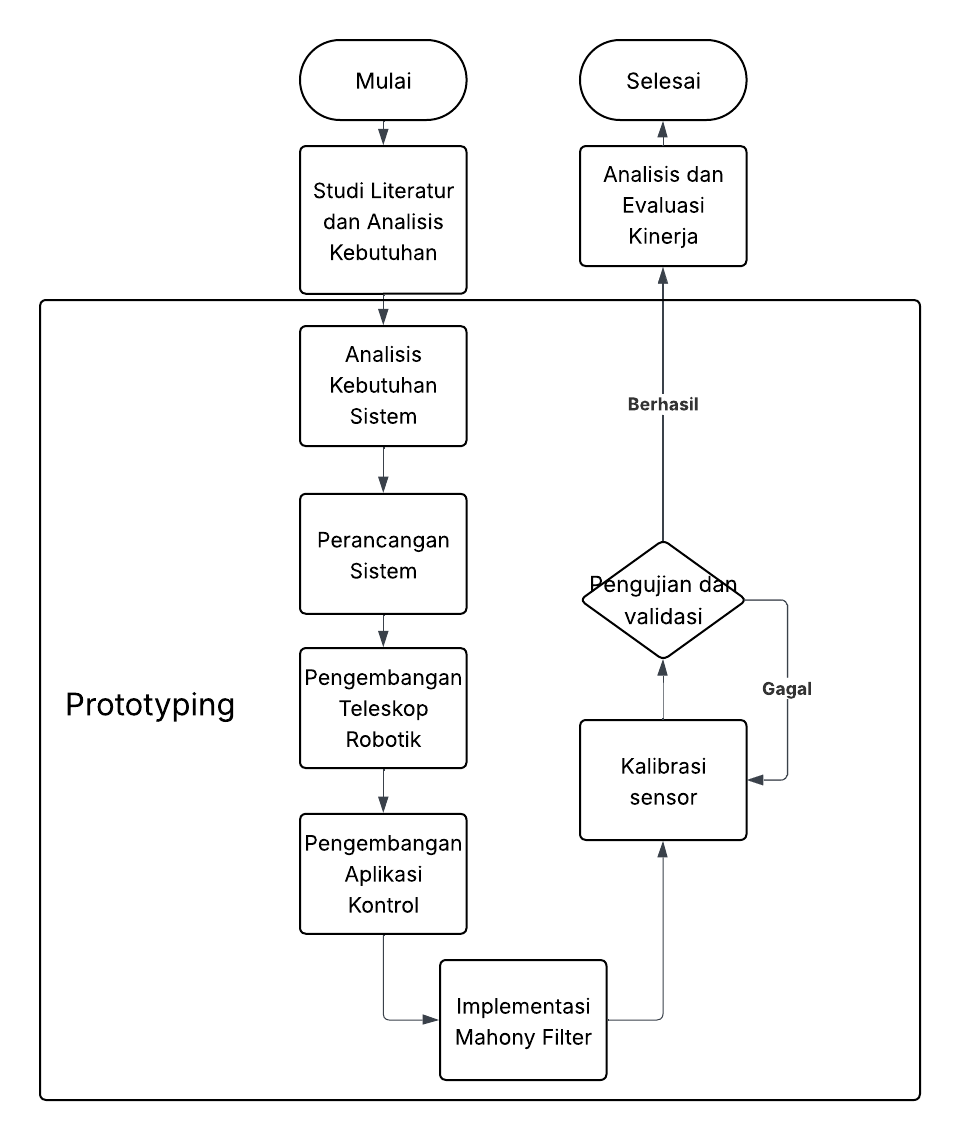
\includegraphics[width=0.7\textwidth]{figure/alur_penelitian.png}
    \caption{Implementasi Fisik Sistem Mekanik Teleskop Robotik}
    \label{fig:4.mounting_mechanical}
\end{figure}

Desain mekanik memperhitungkan distribusi beban dengan menempatkan pusat massa OTA sedekat mungkin dengan titik tumpu untuk mengurangi momen gaya yang harus ditahan oleh motor stepper, disisi sebrang teleskop ditambahkan pemberat untuk mengatur titik berat supaya berada pada posisi seimbang seperti ditunjukkan pada Gambar~\ref{fig:4.mounting_balance}. Material PLA 2+ dipilih karena memiliki kekakuan yang lebih baik dibanding PLA standar dan lebih tahan terhadap deformasi akibat beban statis maupun getaran.

\begin{figure}[H]
    \centering
    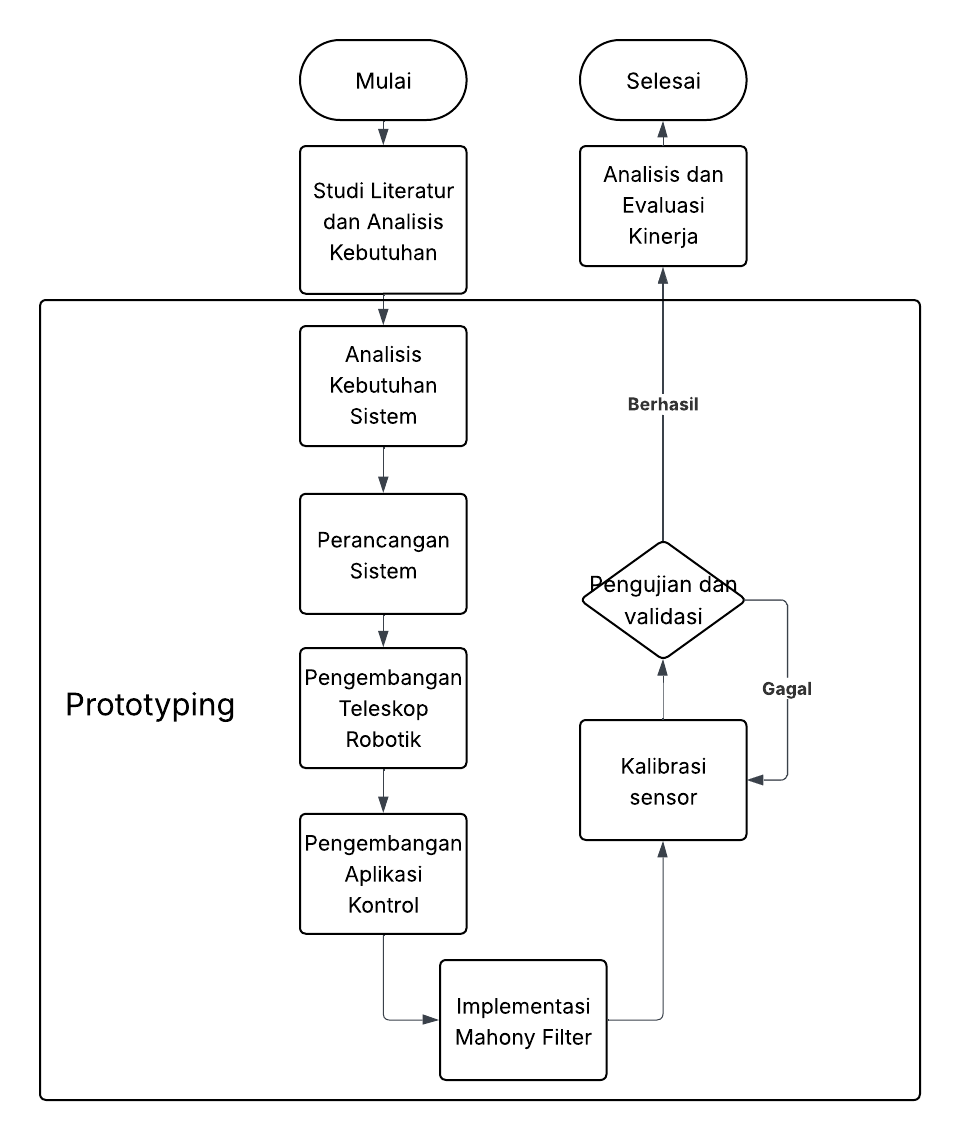
\includegraphics[width=0.7\textwidth]{figure/alur_penelitian.png}
    \caption{Implementasi Fisik Sistem Mekanik Teleskop Robotik}
    \label{fig:4.mounting_balance}
\end{figure}

\subsubsection{Sistem Penggerak}
Sistem transmisi menggunakan motor stepper NEMA 17 dengan resolusi 200 langkah per revolusi (1.8$^{\circ}$ per langkah). Untuk meningkatkan kehalusan gerakan dan mengurangi getaran, Ditambahkan \textit{planetary gear} dengan 4 \textit{stack} ditunjukkan pada Gambar~\ref{fig:4.transmission_system} dan untuk setiap \textit{stack}-nya meningkatkan torsi sebesar 4 kali dan rasio perputarannya menjadi 4 kali untuk 1 putaran. Rasio transmisi menghasilkan resolusi akhir sebesar 69120 langkah untuk satu rotasi penuh sumbu teleskop (360$^{\circ}$), yang setara dengan 192 langkah per derajat atau sekitar 0.00521$^{\circ}$ per langkah. Resolusi ini memadai untuk aplikasi \textit{GoTo} dan \textit{tracking} objek langit dengan diameter sudut semu kecil seperti planet dan bintang.

\begin{figure}[H]
    \centering
    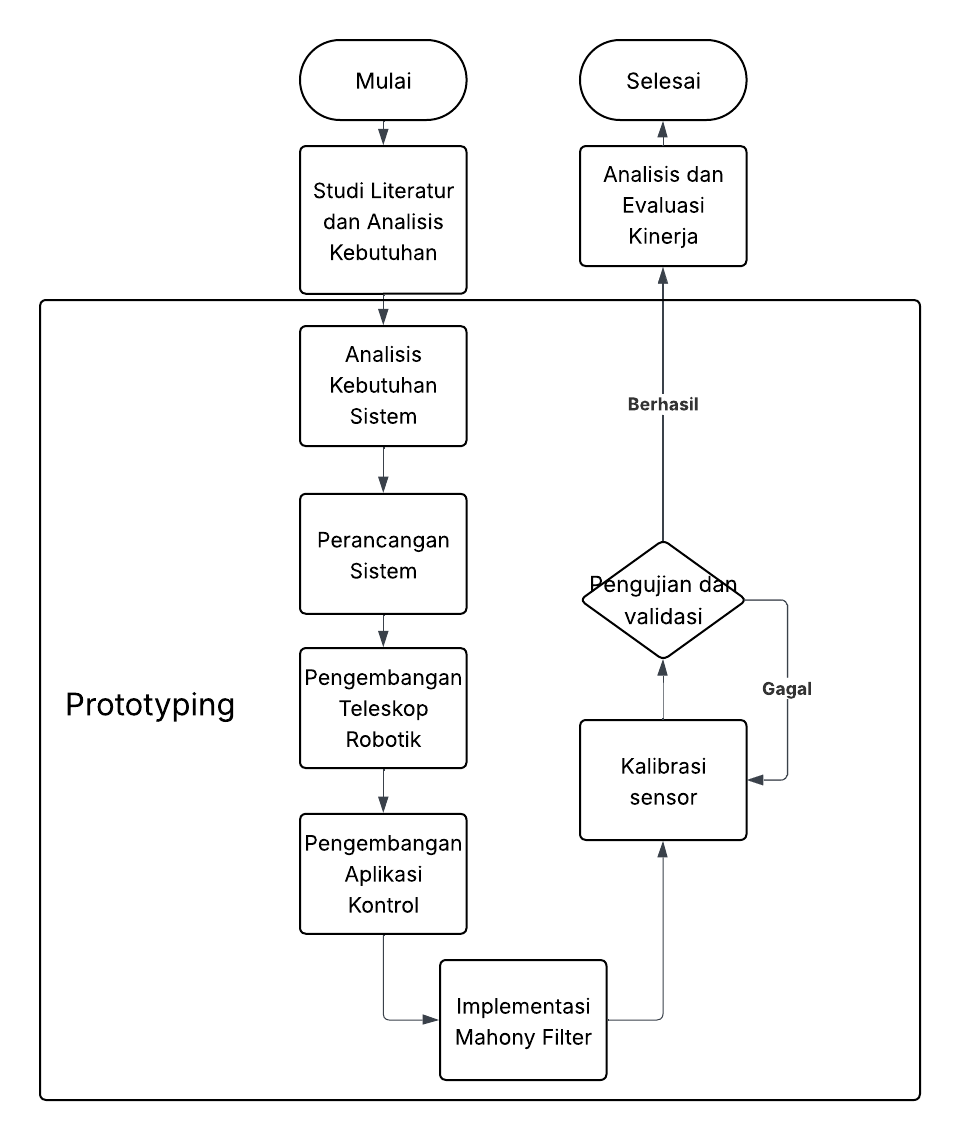
\includegraphics[width=0.65\textwidth]{figure/alur_penelitian.png}
    \caption{Sistem Transmisi Motor Stepper NEMA 17 dengan Belt/Gear}
    \label{fig:4.transmission_system}
\end{figure}

\subsubsection{Mikrokontroler ESP32}
Mikrokontroler ESP32 berfungsi sebagai unit pemrosesan pusat yang menjalankan algoritma fusi sensor, perhitungan koordinat astronomi, dan kendali motor secara real-time. ESP32 dipilih karena memiliki prosesor \textit{dual-core} Xtensa LX6 dengan kecepatan hingga 240~MHz, memori RAM 520~KB, dan dukungan komunikasi WiFi terintegrasi yang memungkinkan kendali teleskop melalui aplikasi Android tanpa memerlukan modul WiFi eksternal. \par

Pada implementasi ini, ESP32 menjalankan dua \textit{task} paralel: (1) \textit{task} pembacaan sensor yang berjalan pada \textit{core} 0 dengan target frekuensi 100~Hz untuk memastikan data orientasi selalu ter-\textit{update}, dan (2) \textit{task} kendali motor dan komunikasi WebSocket yang berjalan pada \textit{core} 1 untuk menangani perintah pengguna dan eksekusi gerakan motor.

\begin{figure}[H]
    \centering
    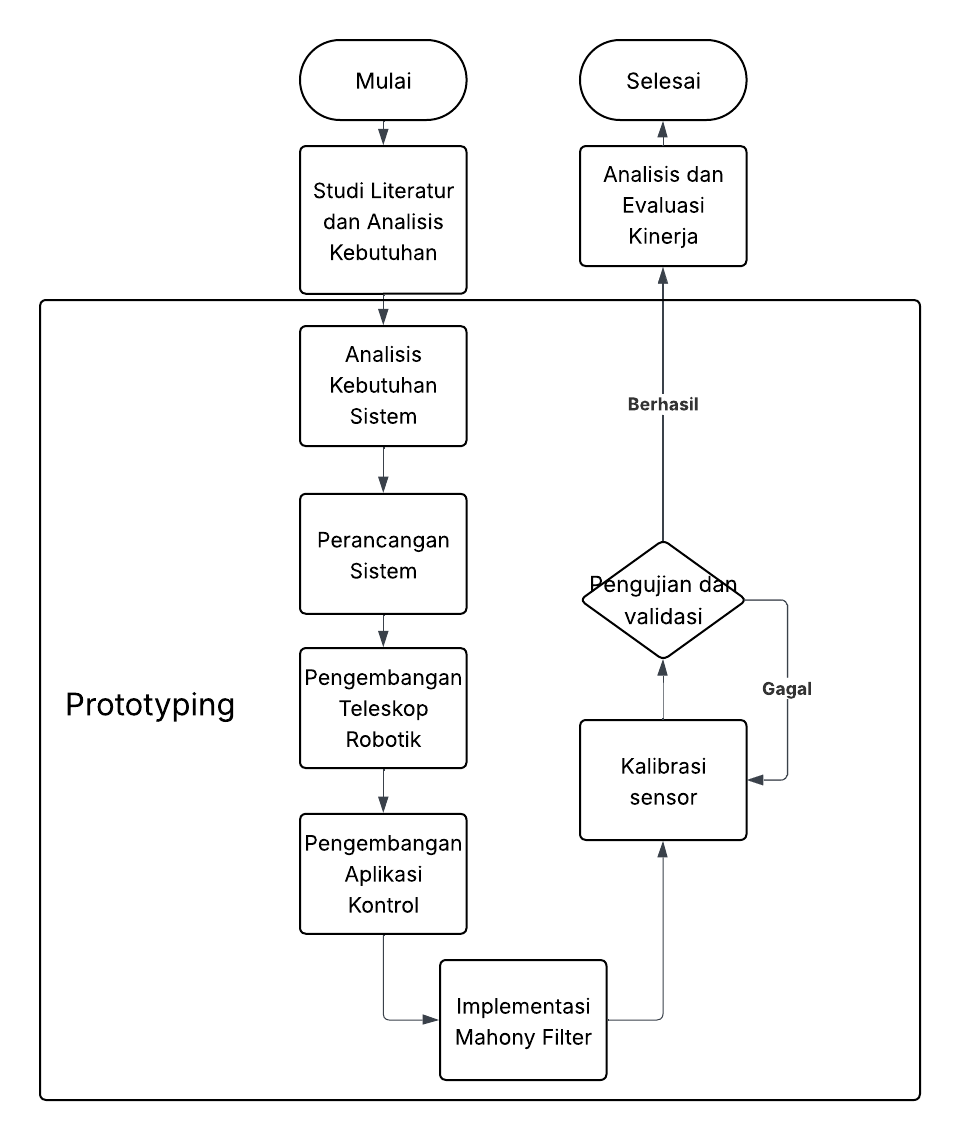
\includegraphics[width=0.5\textwidth]{figure/alur_penelitian.png}
    \caption{Mikrokontroler ESP32 sebagai Unit Pemrosesan Pusat}
    \label{fig:4.esp32_controller}
\end{figure}

\subsubsection{Driver Motor A4988}
Driver motor A4988 merupakan \textit{stepper motor driver} yang mengendalikan dua motor NEMA 17 untuk sumbu \textit{Azimuth} dan \textit{Altitude}. Driver ini mendukung berbagai mode \textit{microstepping} (1/2, 1/4, 1/8, hingga 1/16) yang dikonfigurasi melalui pin MS1, MS2, dan MS3. Pada implementasi ini, mode 1/16 dipilih untuk menghasilkan gerakan yang lebih halus dan mengurangi \textit{resonance} motor pada kecepatan rendah. \par

Driver A4988 dilengkapi dengan proteksi arus berlebih dan proteksi temperatur yang melindungi motor dari kerusakan. Arus motor diatur melalui potensiometer onboard dengan nilai referensi tegangan $V_{ref}$ yang disesuaikan dengan spesifikasi motor NEMA 17 yang digunakan (umumnya 1--1.5~A per fase).

\begin{figure}[H]
    \centering
    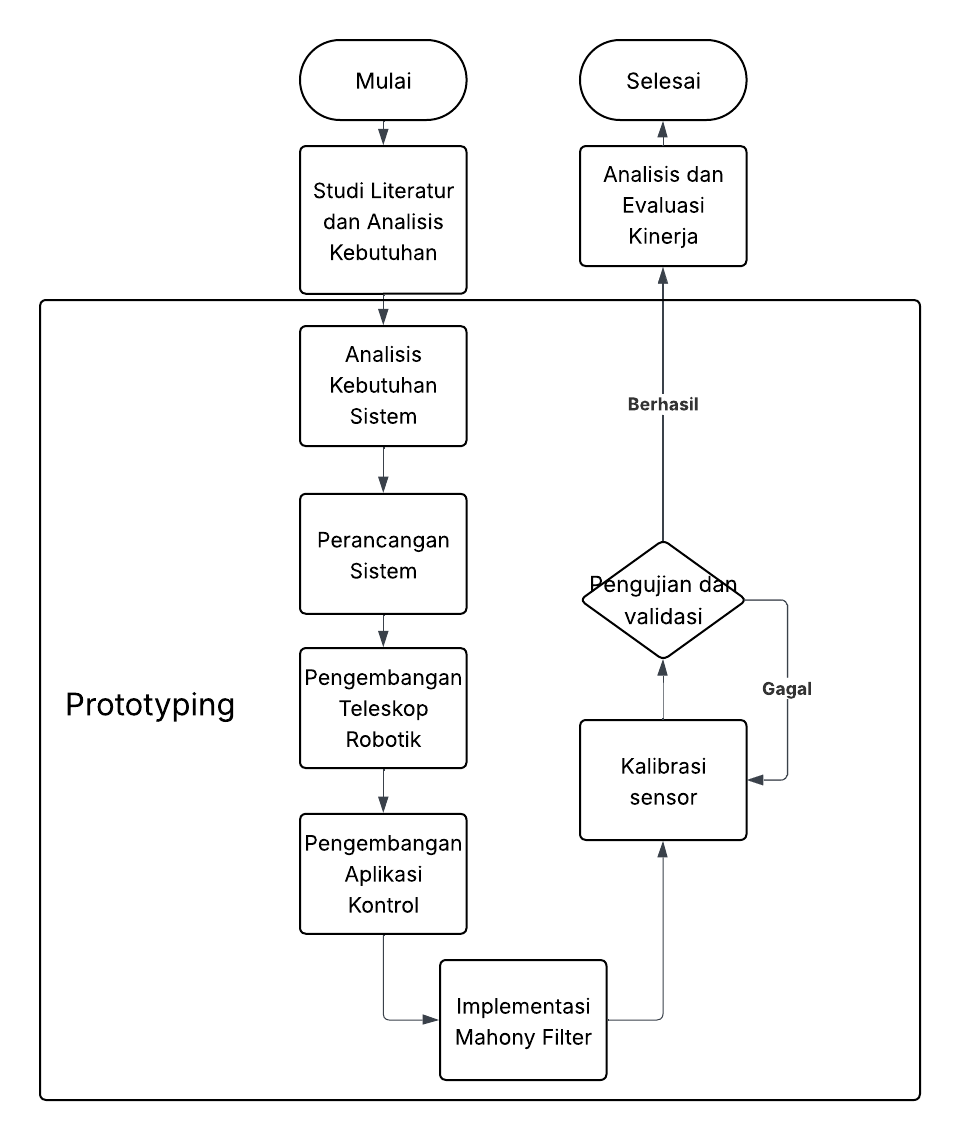
\includegraphics[width=0.55\textwidth]{figure/alur_penelitian.png}
    \caption{Driver Motor A4988 untuk Kendali Motor Stepper}
    \label{fig:4.motor_driver}
\end{figure}

\subsubsection{Sensor IMU MPU6050}
MPU6050 merupakan sensor \textit{Inertial Measurement Unit} (IMU) 6-axis yang menggabungkan akselerometer 3-axis dan giroskop 3-axis dalam satu chip. Sensor ini digunakan untuk mengukur orientasi teleskop dalam bentuk sudut \textit{roll} dan \textit{pitch} yang kemudian digunakan dalam algoritma \textit{tilt compensation} untuk kompensasi kemiringan pembacaan kompas magnetik. \par

MPU6050 berkomunikasi dengan ESP32 melalui protokol I$^2$C dengan alamat default 0x68. Sensor ini memiliki rentang pengukuran akselerometer yang dapat dikonfigurasi ($\pm$2g, $\pm$4g, $\pm$8g, $\pm$16g) dan rentang giroskop ($\pm$250$^{\circ}$/s, $\pm$500$^{\circ}$/s, $\pm$1000$^{\circ}$/s, $\pm$2000$^{\circ}$/s). Pada implementasi ini, akselerometer dikonfigurasi pada $\pm$2g dan giroskop pada $\pm$250$^{\circ}$/s untuk mendapatkan resolusi pembacaan maksimal sesuai dengan rentang gerakan teleskop yang relatif lambat.

\begin{figure}[H]
    \centering
    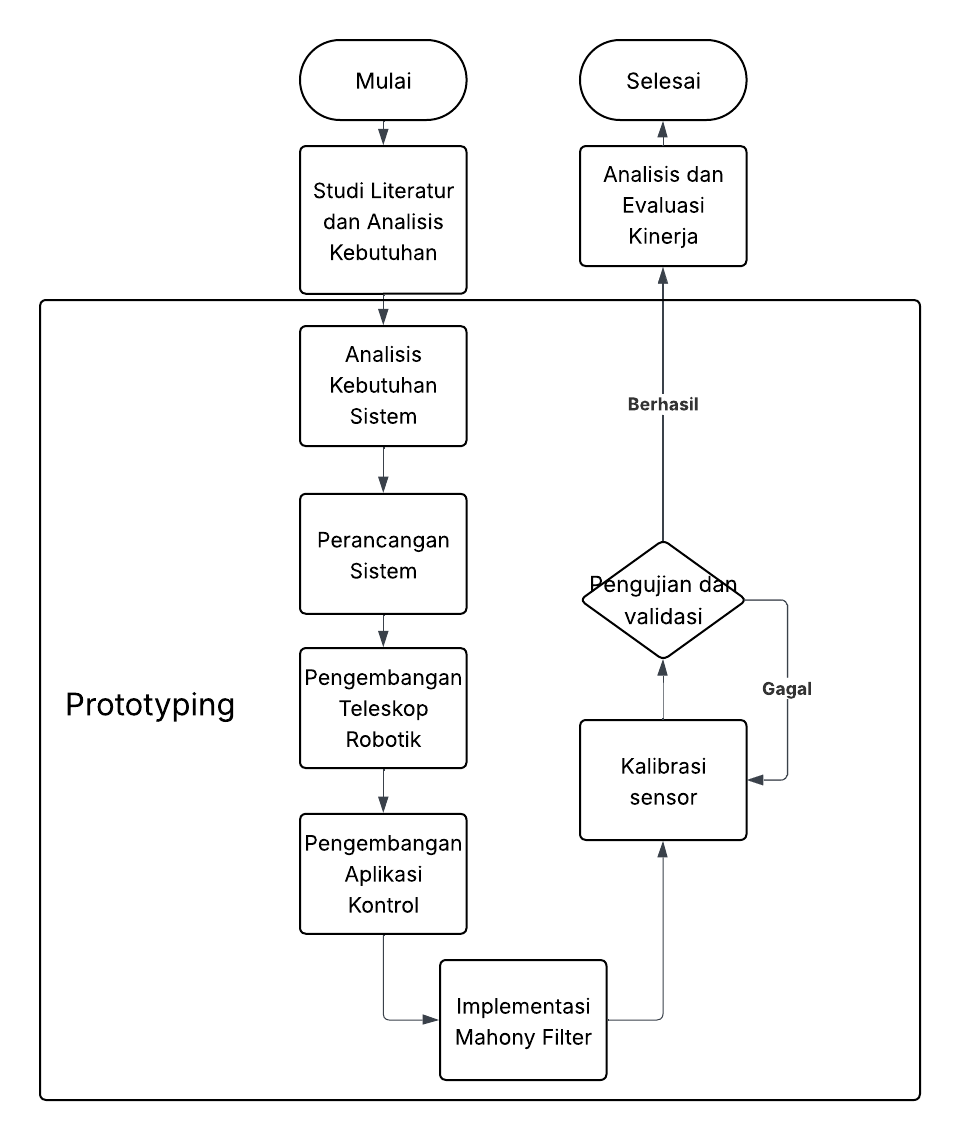
\includegraphics[width=0.5\textwidth]{figure/alur_penelitian.png}
    \caption{Sensor IMU MPU6050 untuk Pengukuran Orientasi}
    \label{fig:4.mpu6050}
\end{figure}

\subsubsection{Sensor Magnetometer QMC5883L}
QMC5883L adalah sensor magnetometer 3-axis yang digunakan untuk mengukur medan magnet bumi dan menentukan arah \textit{heading} (azimuth) absolut terhadap utara magnetik. Sensor ini menggantikan kompas mekanik tradisional dan memberikan pembacaan digital dengan resolusi tinggi melalui protokol I$^2$C (alamat default 0x0D). \par

Dalam implementasi, QMC5883L digunakan pada tahap inisialisasi sistem untuk menentukan referensi arah utara. Setelah sistem mendapatkan referensi awal melalui \textit{tilt-compensated heading}, pembacaan \textit{azimuth} operasional dialihkan ke encoder AS5600 yang lebih stabil terhadap interferensi elektromagnetik dari motor stepper. Sensor ini memiliki rentang pengukuran $\pm$8 Gauss dan resolusi output 16-bit per sumbu.

\begin{figure}[H]
    \centering
    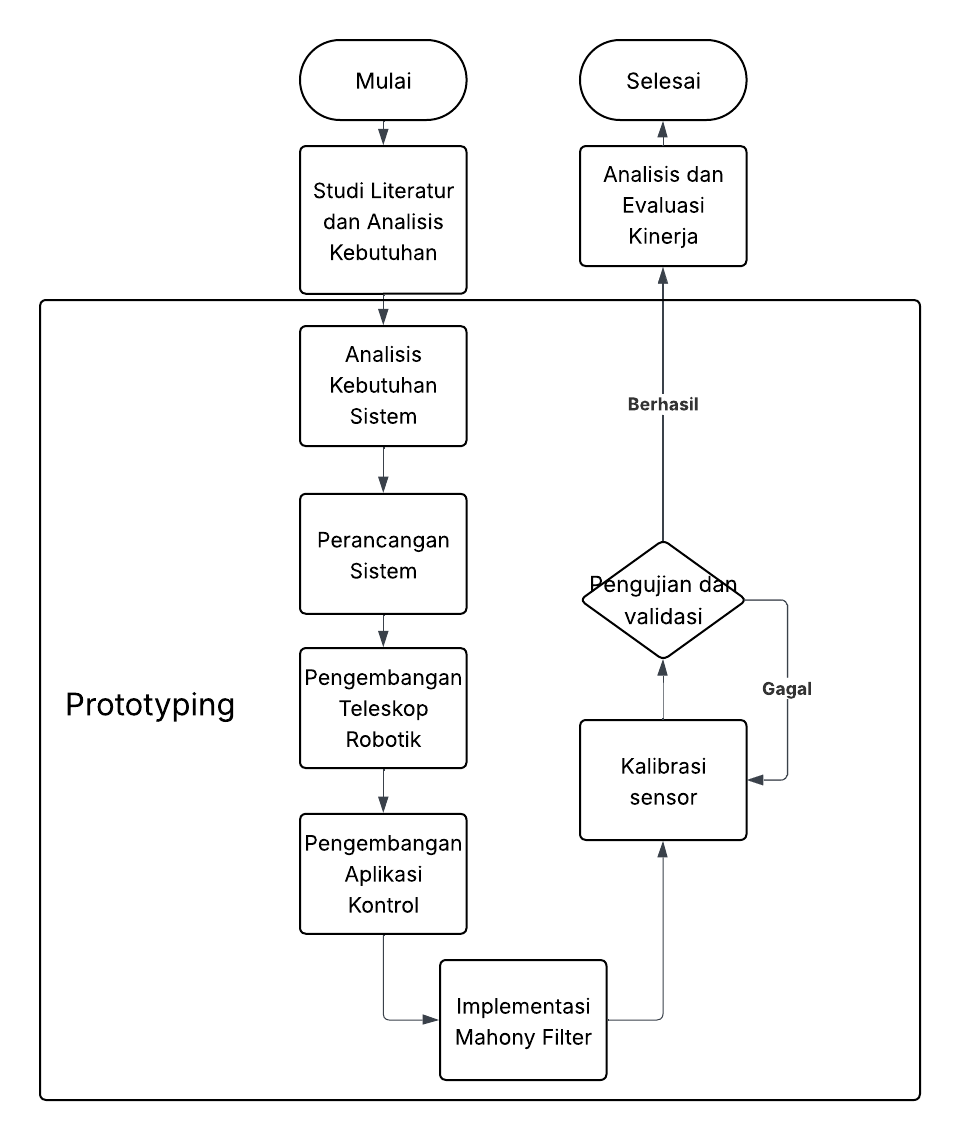
\includegraphics[width=0.5\textwidth]{figure/alur_penelitian.png}
    \caption{Sensor Magnetometer QMC5883L untuk Referensi Arah Utara}
    \label{fig:4.qmc5883l}
\end{figure}

\subsubsection{Encoder Magnetik AS5600}
AS5600 merupakan encoder magnetik 12-bit \textit{contactless} yang memberikan pembacaan posisi sudut absolut dengan resolusi 4096 langkah per rotasi (360$^{\circ}$/4096 $\approx$ 0.088$^{\circ}$ per langkah). Sistem menggunakan dua buah encoder AS5600: satu untuk sumbu \textit{Azimuth} dan satu untuk sumbu \textit{Altitude}. Encoder ini bekerja dengan mendeteksi orientasi medan magnet dari magnet diametral yang dipasang pada poros rotasi sumbu. \par

Keunggulan AS5600 dibanding encoder optik adalah ketahanannya terhadap debu dan tidak memerlukan kontak mekanik, sehingga lebih awet dan bebas perawatan. Sensor ini berkomunikasi melalui I$^2$C dan dapat dikonfigurasi untuk memberikan output sudut dalam format mentah (raw angle) atau sudut yang sudah dikalibrasi. Pada implementasi, pembacaan \textit{raw angle} digunakan dan offset kalibrasi diterapkan pada \textit{firmware} untuk fleksibilitas penyesuaian.

\begin{figure}[H]
    \centering
    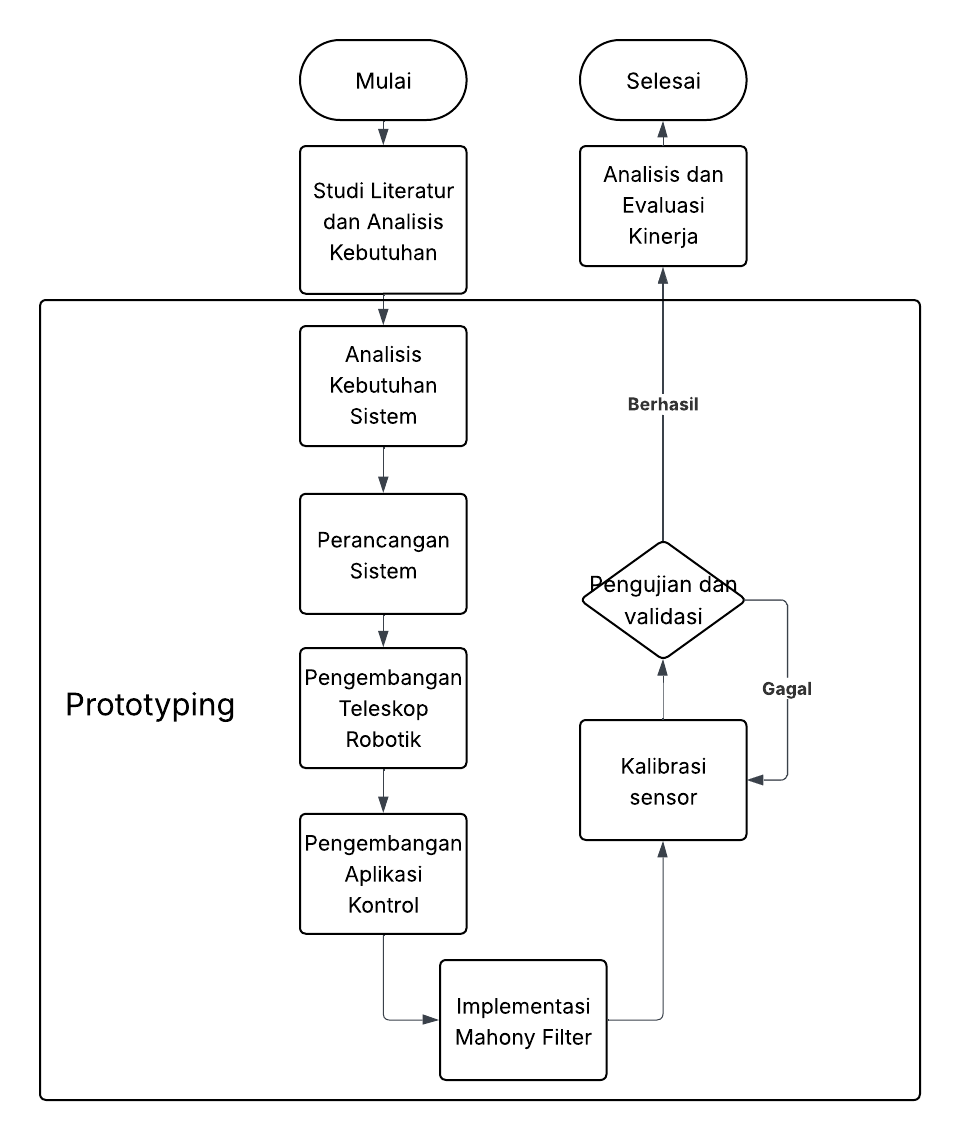
\includegraphics[width=0.55\textwidth]{figure/alur_penelitian.png}
    \caption{Encoder Magnetik AS5600 untuk Pembacaan Sudut Absolut}
    \label{fig:4.as5600}
\end{figure}

\subsubsection{Integrasi Sistem Elektronik}
Seluruh komponen elektronik dipusatkan pada \textit{enclosure} yang dirancang untuk melindungi rangkaian dari debu dan kelembaban. Sistem catu daya menggunakan adaptor 12V DC yang mendistribusikan tegangan ke driver motor A4988 (12V) dan regulator step-down untuk menyuplai ESP32 dan sensor-sensor (3.3V dan 5V). Jalur komunikasi I$^2$C digunakan bersama oleh MPU6050, QMC5883L, dan dua buah AS5600 dengan alamat yang berbeda atau melalui multiplexer I$^2$C jika diperlukan. \par

Tata letak komponen dalam \textit{enclosure} mempertimbangkan pemisahan jalur daya motor (yang menghasilkan \textit{noise} elektromagnetik tinggi) dari jalur sinyal sensor untuk meminimalkan interferensi. Kabel sensor menggunakan kabel \textit{twisted pair} dan dijauhkan dari kabel motor. Grounding sistem dilakukan pada satu titik \textit{common ground} untuk mencegah \textit{ground loop} yang dapat menimbulkan \textit{noise} pada pembacaan sensor analog.

\begin{figure}[H]
    \centering
    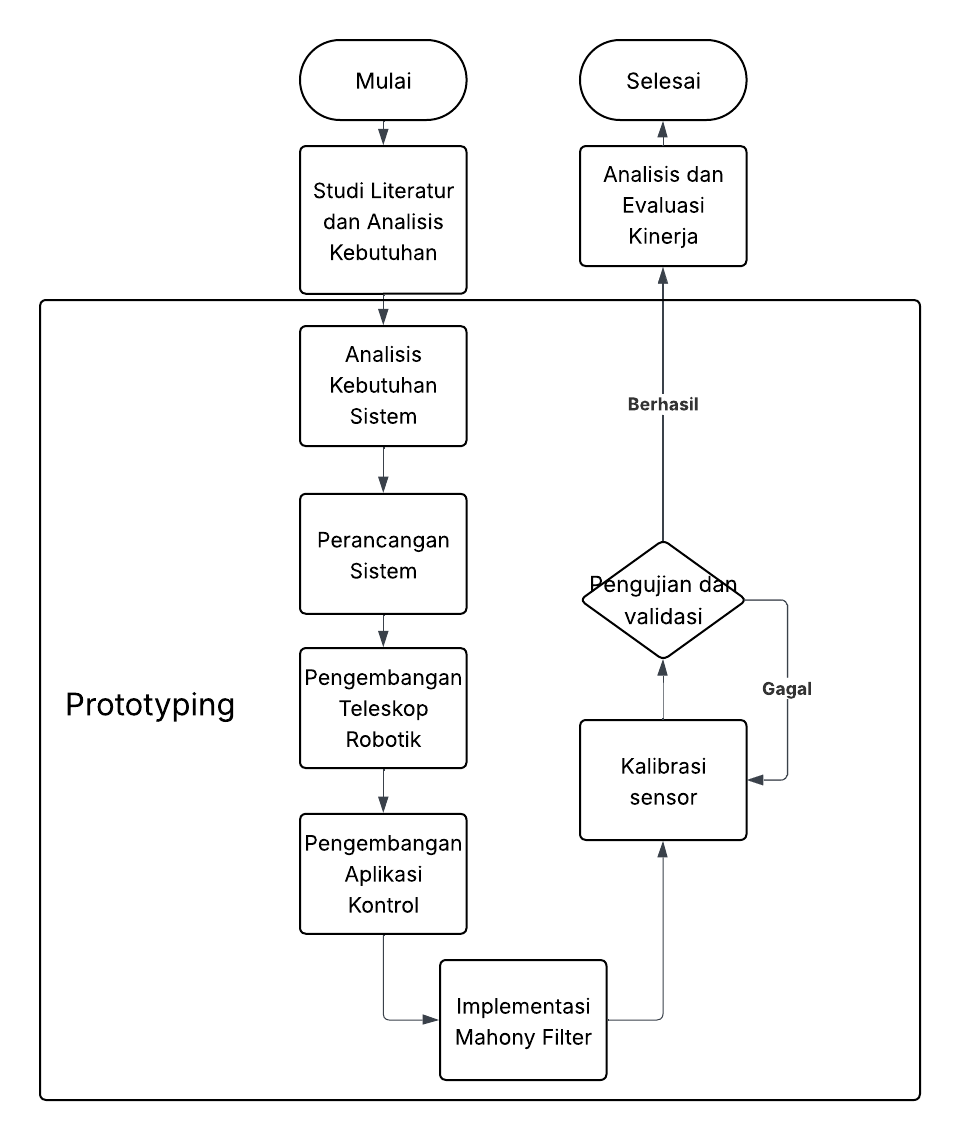
\includegraphics[width=0.7\textwidth]{figure/alur_penelitian.png}
    \caption{Integrasi Sistem Elektronik dalam \textit{Enclosure}}
    \label{fig:4.electronics_integration}
\end{figure}

\subsection{Implementasi Perangkat Lunak dan Algoritma} \label{IV.Software}
Perangkat lunak (\textit{firmware}) berperan vital dalam menerjemahkan data sensor yang \textit{raw} dan \textit{noisy} menjadi informasi orientasi yang stabil. Berdasarkan implementasi program pada mikrokontroler, alur utama sistem terdiri dari dua bagian: (1) \textit{task} pembacaan sensor yang berjalan periodik, dan (2) \textit{loop} kendali motor serta komunikasi yang berjalan kontinu. \par

Algoritma utama yang digunakan adalah fusi sensor. Kode sumber lengkap dapat dilihat pada lampiran, namun berikut adalah penjabaran logika utama dalam bentuk \textit{pseudocode}:

\begin{lstlisting}[caption={Pseudocode Alur Sensor dan Orientasi (Ringkas)}, label={code:4.pseudocode_main}, language=C]
// Sensor loop (target 100 Hz)
loopSensor() {
    // 1) Baca IMU MPU6050
    ax, ay, az, gx, gy, gz = readMPU6050();

    // 2) Mahony filter (hanya jika akselerasi masuk akal)
    if (0.25 <= (ax^2+ay^2+az^2) <= 4.0) {
        MahonyUpdate(gx, gy, gz, ax, ay, az, dt);
    }
    pitch = MahonyPitch() - pitchCorrection;
    roll  = MahonyRoll()  - rollCorrection;

    // 3) Inisialisasi azimuth absolut sekali via kompas (tilt compensation)
    //    lalu simpan offset terhadap encoder azimuth (deltaAzimuth)
    if (deltaAzimuth is NaN) {
        mx, my, mz = readQMC5883L();
        heading = tiltCompensatedHeading(mx, my, mz, roll, pitch);
        deltaAzimuth = readAzimuthEncoder() - heading;
    }

    // 4) Operasional harian: azimuth dan altitude dari dua encoder AS5600
    azimuth  = readAzimuthEncoder() - deltaAzimuth;
    altitude = readAltitudeEncoder() - altitudeOffset;
}
\end{lstlisting}

Pseudocode pada Kode \ref{code:4.pseudocode_main} merangkum implementasi aktual: Mahony Filter digunakan untuk menghasilkan \textit{pitch} dan \textit{roll} yang stabil dari MPU6050 \cite{Mahony2007,Maton2024}. Sementara itu, sensor kompas QMC5883L berfungsi sebagai acuan arah absolut untuk mendapatkan referensi \textit{Azimuth} pada saat inisialisasi (melalui \textit{tilt compensation}), kemudian sistem bergantung pada pembacaan encoder AS5600 untuk \textit{Azimuth} dan \textit{Altitude} agar lebih stabil terhadap \textit{noise} sesaat dan gangguan elektromagnetik dari motor. \par

Bagian berikut melengkapi pseudocode dengan: (1) perhitungan koordinat target (bintang/matahari/bulan/planet) hingga \textit{Altitude-Azimuth}, dan (2) konversi sudut target menjadi langkah motor stepper. Transformasi koordinat astronomi yang digunakan mengikuti konsep waktu sideris lokal, sudut jam, dan konversi koordinat ekuatorial--horizontal \cite{Roy2018,HannuKarttunen2017}. \par

\subsubsection{Perhitungan Posisi Benda Langit (Bintang/Matahari/Bulan/Planet)} \label{IV.Software.Astro}
Pada mode \textit{GoTo}, sistem membentuk target \textit{Altitude} dan \textit{Azimuth} dari input lokasi (lintang, bujur) dan waktu RTC. Untuk bintang, nilai \textit{Right Ascension} (RA) dan \textit{Declination} (Dec) diperoleh dari perintah aplikasi (mis. dari \textit{planetarium software}), sedangkan untuk Matahari, Bulan, dan Planet, RA/Dec dihitung secara \textit{on-device} menggunakan model aproksimasi. \par

\begin{lstlisting}[caption={Pseudocode Perhitungan Target Altitude-Azimuth (UpdateTarget)}, label={code:4.pseudocode_target_altaz}, language=C]
updateTarget() {
    if (selectedRA or selectedDec is NaN) return;

    // 1) Hitung Julian Date dari waktu RTC
    JD = julianDate(year, month, day, hour, minute, second);

    // 2) Hitung Local Sidereal Time (LST) dari JD dan bujur
    LST = localSiderealTime(longitude, JD);    // derajat

    // 3) Tentukan koordinat ekuatorial (RA/Dec) target
    //    Catatan: RA dari ephemeris sering diperoleh dalam derajat (0-360)
    //    sehingga perlu konversi raHour = raDeg/15 sebelum dipakai pada calcAltAz.
    if (objectType == SUN)    { (raDeg, decDeg) = calcSunRaDec(JD);    raHour = raDeg/15.0; }
    if (objectType == MOON)   { (raDeg, decDeg) = calcMoonRaDec(JD);   raHour = raDeg/15.0; }
    if (objectType == PLANET) { (raDeg, decDeg) = calcPlanetRaDec(planetIndex, JD); raHour = raDeg/15.0; }
    if (objectType == STAR) {
        // dari aplikasi: selectedRA dalam jam (0-24), selectedDec dalam derajat
        raHour = selectedRA;
        decDeg = selectedDec;
        raDeg  = raHour * 15.0;
    }

    // 4) Konversi (RA/Dec) -> (Alt/Az) sesuai lintang dan LST
    (targetAltDeg, targetAzDeg) = calcAltAz(latitude, decDeg, raHour, LST);

    // 5) Kirim target ke kendali motor
    moveMotor(targetAzDeg, targetAltDeg);
}
\end{lstlisting}

\subsubsection{Transformasi Koordinat: Julian Date, LST, dan Altitude-Azimuth} \label{IV.Software.Transform}
Fungsi astronomi pada firmware terdiri dari perhitungan Julian Date ($JD$), waktu sideris lokal ($LST$), dan konversi koordinat ekuatorial (RA/Dec) menjadi koordinat horizontal (Alt/Az). Pada implementasi, $LST$ dinyatakan dalam derajat, sedangkan RA dari antarmuka dinyatakan dalam jam sehingga perlu konversi $RA_{deg}=15\cdot RA_{hour}$. \par

\begin{lstlisting}[caption={Pseudocode Inti Transformasi Koordinat Astronomi}, label={code:4.pseudocode_astro_math}, language=C]
// Julian Date
julianDate(y, m, d, hh, mm, ss) {
    if (m <= 2) { y -= 1; m += 12; }
    A = floor(y/100);
    B = 2 - A + floor(A/4);
    JD0 = floor(365.25*(y+4716)) + floor(30.6001*(m+1)) + d + B - 1524.5;
    dayFrac = (hh + mm/60 + ss/3600) / 24;
    return JD0 + dayFrac;
}

// Local Sidereal Time (derajat)
localSiderealTime(longDeg, JD) {
    T = (JD - 2451545.0)/36525.0;
    GST = 280.46061837 + 360.98564736629*(JD-2451545.0)
          + 0.000387933*T*T - (T*T*T)/38710000.0;
    GST = wrap360(GST);
    LST = wrap360(GST + longDeg);
    return LST;
}

// Ekuatorial -> Horizontal
calcAltAz(latDeg, decDeg, raHour, lstDeg) {
    HAdeg = wrap180(lstDeg - 15*raHour);   // hour angle (deg), dibatasi [-180,180]
    HA = radians(HAdeg);
    lat = radians(latDeg);
    dec = radians(decDeg);

    // altitude
    sinAlt = sin(lat)*sin(dec) + cos(lat)*cos(dec)*cos(HA);
    alt = asin(sinAlt);

    // azimuth (pakai acos + koreksi kuadran dengan sin(HA))
    cosAz = (sin(dec) - sin(lat)*sin(alt)) / (cos(lat)*cos(alt));
    az = acos(clamp(cosAz, -1, 1));
    if (sin(HA) > 0) az = 2*pi - az;

    return (degrees(alt), degrees(az));
}
\end{lstlisting}

Bagian ini menjelaskan fungsi perhitungan koordinat ekuatorial (RA/Dec) untuk objek dinamis. Pada sistem ini, \textbf{bintang} menggunakan RA/Dec dari aplikasi, sedangkan \textbf{Matahari, Bulan, dan Planet} dihitung secara \textit{on-device} berdasarkan waktu (RTC) yang dikonversi ke $JD$. Hasil RA/Dec kemudian digunakan pada Kode \ref{code:4.pseudocode_target_altaz} untuk menghasilkan target \textit{Altitude} dan \textit{Azimuth}. \par

\subsubsection{Perhitungan RA/Dec Matahari (\texttt{calcSunRaDec})} \label{IV.Software.SunRaDec}
Fungsi \texttt{calcSunRaDec} menghitung RA/Dec Matahari dengan tahapan: menghitung abad Julian $T$, menentukan bujur rata-rata Matahari ($L_0$), anomali rata-rata ($M$), dan \textit{equation of center} ($C$) untuk memperoleh bujur ekliptika sebenarnya ($\lambda$). Selanjutnya, koordinat ekliptika dikonversi ke koordinat ekuatorial menggunakan kemiringan ekliptika ($\varepsilon$). Keluaran fungsi adalah $(RA,Dec)$ dalam derajat, dengan $RA\in[0,360)$. \par

\begin{lstlisting}[caption={Pseudocode Perhitungan RA/Dec Matahari (calcSunRaDec)}, label={code:4.pseudocode_sun_radec}, language=C]
calcSunRaDec(JD) {
    T = (JD - 2451545.0)/36525.0;
    L0 = wrap360(280.46646 + 36000.76983*T + 0.0003032*T*T);
    M  = radians(wrap360(357.52911 + 35999.05029*T - 0.0001537*T*T));
    C  = (1.914602 - 0.004817*T)*sin(M) + 0.019993*sin(2M) + 0.000289*sin(3M);
    lambda = radians(L0 + C);
    eps = radians(23.439291 - 0.0130042*T);
    dec = asin( sin(eps)*sin(lambda) );
    ra  = atan2( cos(eps)*sin(lambda), cos(lambda) );
    return (wrap360(degrees(ra)), degrees(dec));
}
\end{lstlisting}

\subsubsection{Perhitungan RA/Dec Bulan (\texttt{calcMoonRaDec})} \label{IV.Software.MoonRaDec}
Fungsi \texttt{calcMoonRaDec} menggunakan aproksimasi orde rendah: menghitung argumen fundamental Bulan ($L_0, M, M_m, F$), lalu membentuk bujur ekliptika ($\lambda$) dan lintang ekliptika ($\beta$). Selanjutnya, $(\lambda,\beta)$ dikonversi ke vektor ekuatorial $(x,y,z)$ menggunakan kemiringan ekliptika $\varepsilon$, dan RA/Dec diperoleh dari \textit{atan2} dan \textit{asin}. Pendekatan ini memadai untuk kebutuhan \textit{GoTo} pada skala derajat, namun tidak ditujukan untuk presisi tinggi (mis. koreksi paralaks/toposentrik detail). \par

\begin{lstlisting}[caption={Pseudocode Perhitungan RA/Dec Bulan (calcMoonRaDec, aproksimasi)}, label={code:4.pseudocode_moon_radec}, language=C]
calcMoonRaDec(JD) {
    T = (JD - 2451545.0)/36525.0;

    L0 = radians(wrap360(
          218.3164477
        + 481267.88123421*T
        - 0.00015786*T*T
        + (T*T*T)/538841.0
        - (T*T*T*T)/65194000.0));

    M  = radians(wrap360(
          357.5291092
        + 35999.0502909*T
        - 0.0001536*T*T
        + (T*T*T)/24490000.0));

    Mm = radians(wrap360(
          134.9633964
        + 477198.8675055*T
        + 0.0087414*T*T
        + (T*T*T)/69699.0
        - (T*T*T*T)/14712000.0));

    F  = radians(wrap360(
          93.2720950
        + 483202.0175233*T
        - 0.0036539*T*T
        - (T*T*T)/3526000.0
        + (T*T*T*T)/863310000.0));

    lambda = L0
           + radians(6.289)*sin(Mm)
           + radians(1.274)*sin(2*L0 - Mm)
           + radians(0.658)*sin(2*L0)
           + radians(0.214)*sin(2*Mm)
           - radians(0.186)*sin(M);

    beta = radians(5.128)*sin(F)
         + radians(0.280)*sin(Mm + F)
         + radians(0.277)*sin(Mm - F);

    eps = radians(23.43929111 - 0.013004167*T);

    x = cos(lambda)*cos(beta);
    y = sin(lambda)*cos(beta)*cos(eps) - sin(beta)*sin(eps);
    z = sin(lambda)*cos(beta)*sin(eps) + sin(beta)*cos(eps);

    ra  = atan2(y, x);
    dec = asin(z);
    return (wrap360(degrees(ra)), degrees(dec));
}
\end{lstlisting}

\subsubsection{Perhitungan RA/Dec Planet (\texttt{calcPlanetRaDec})} \label{IV.Software.PlanetRaDec}
Fungsi \texttt{calcPlanetRaDec} menggunakan parameter orbit sederhana tiap planet (semi-mayor $a$, eksentrisitas $e$, bujur rata-rata $L$, dan bujur perihelion $\bar{\omega}$). Nilai anomali rata-rata $M$ dihitung dari $L-\bar{\omega}$, kemudian eksentrik anomali $E$ diselesaikan secara iteratif (beberapa iterasi cukup untuk pendekatan ini). Setelah itu dihitung \textit{true anomaly} $v$ dan posisi relatif pada bidang ekliptika, lalu dipetakan ke koordinat ekuatorial menggunakan kemiringan ekliptika. Model ini merupakan aproksimasi untuk kebutuhan \textit{GoTo} dan belum memasukkan koreksi perturbasi dan model heliosentrik/geosentrik lengkap. \par

\begin{lstlisting}[caption={Pseudocode Perhitungan RA/Dec Planet (calcPlanetRaDec, aproksimasi)}, label={code:4.pseudocode_planet_radec}, language=C]
calcPlanetRaDec(index, JD) {
    p = planets[index];

    M = radians(wrap360(p.L - p.w_bar));

    E = M;
    for (int i = 0; i < 5; i++) {
        E = M + p.e*sin(E);
    }

    xv = cos(E) - p.e;
    yv = sqrt(1 - p.e*p.e) * sin(E);
    v  = atan2(yv, xv);
    r  = sqrt(xv*xv + yv*yv);

    lon = v + radians(p.w_bar);
    eps = radians(23.439291);

    x = r*cos(lon);
    y = r*cos(eps)*sin(lon);
    z = r*sin(eps)*sin(lon);

    ra  = atan2(y, x);
    dec = atan2(z, sqrt(x*x + y*y));
    return (wrap360(degrees(ra)), degrees(dec));
}
\end{lstlisting}

\subsubsection{Tilt Compensation untuk Heading Kompas} \label{IV.Software.CompassTilt}
Untuk mengurangi kesalahan \textit{heading} kompas akibat kemiringan pemasangan sensor, dilakukan \textit{tilt compensation}. Intinya, vektor medan magnet $(m_x,m_y,m_z)$ diproyeksikan ke bidang horizontal menggunakan estimasi \textit{roll} dan \textit{pitch}, lalu \textit{heading} dihitung dengan $\mathrm{atan2}$. \par

\begin{lstlisting}[caption={Pseudocode Tilt-Compensated Heading}, label={code:4.pseudocode_tilt_heading}, language=C]
tiltCompensatedHeading(mx, my, mz, rollDeg, pitchDeg) {
    roll  = radians(rollDeg);
    pitch = radians(pitchDeg);

    Xh = mx*cos(pitch) + mz*sin(pitch);
    Yh = mx*sin(roll)*sin(pitch) + my*cos(roll) - mz*sin(roll)*cos(pitch);

    heading = degrees(atan2(Yh, Xh));
    if (heading < 0) heading += 360;
    return heading;
}
\end{lstlisting}

\subsubsection{Konversi Derajat ke Step Motor dan Logika \textit{GoTo}} \label{IV.Software.Steps}
Konversi sudut ke langkah motor ditentukan oleh total langkah per satu rotasi mekanik sumbu, yang dipengaruhi oleh \textit{step angle} motor, \textit{microstepping}, dan rasio transmisi (jika ada). Pada implementasi, nilai ini disatukan sebagai konstanta \texttt{STEP\_ONE\_ROTATION}. Dengan \texttt{STEP\_ONE\_ROTATION}=69120, maka resolusi teoritis adalah $69120/360=192$ step per derajat (sekitar $0.00521^{\circ}$/step). \par

\begin{lstlisting}[caption={Pseudocode Konversi Sudut ke Step dan Kendali GoTo Motor}, label={code:4.pseudocode_motor_steps}, language=C]
degreeToStep(deg) {
    return round((deg/360) * STEP_ONE_ROTATION);
}

moveMotor(targetAzDeg, targetAltDeg) {
    // Kendali menggunakan umpan balik sudut sensor (encoder)
    currAz = sensorAzimuth;
    deltaAz = targetAzDeg - currAz;
    deltaAz = wrap180(deltaAz);          // pastikan lintasan terpendek

    if (abs(deltaAz) >= AZ_TOLERANCE) {
        stepperAZ.move( degreeToStep(deltaAz) );
    }

    deltaAlt = targetAltDeg - sensorAltitude;
    if (abs(deltaAlt) >= ALT_TOLERANCE) {
        stepperALT.move( degreeToStep(deltaAlt) );
    }
}
\end{lstlisting}

\subsubsection{Ringkasan Tahap Penting Mahony Filter di Firmware} \label{IV.Software.MahonyDetail}
Mahony Filter pada firmware dijalankan pada frekuensi target 100~Hz. Implementasi menerapkan \textit{guard} terhadap nilai $dt$ yang tidak valid ($dt\le 0$ atau terlalu besar), serta hanya memperbarui filter jika norma akselerasi berada dalam rentang wajar (pada kode: $0.25 \le a_x^2+a_y^2+a_z^2 \le 4.0$). Strategi ini membantu mencegah \textit{update} ketika pembacaan akselerometer menyimpang jauh akibat guncangan atau kesalahan baca, sehingga keluaran \textit{roll/pitch} lebih stabil untuk proses \textit{tilt compensation} kompas dan analisis \cite{Mahony2007,Maton2024}. \par

\section{Hasil Pengujian} \label{IV.Hasil_Uji}

Pengujian dilakukan dalam beberapa tahap: pengujian subsistem sensor, pengujian mekanik, dan pengujian lapangan (observasi).

\subsection{Validasi Kebutuhan Sistem (Menjawab Bab~\ref{III.Metode.Uji})} \label{IV.Validasi36}
Subbab ini disusun untuk memastikan Bab IV secara eksplisit \textbf{menjawab Bab~\ref{III.Metode.Uji}} (Pengujian dan Validasi Sistem). Validasi dilakukan dengan memetakan kebutuhan pada Tabel~\ref{table:3.kebutuhanF} (fungsional) dan Tabel~\ref{table:3.kebutuhanNF} (non-fungsional) terhadap hasil pengujian yang dipaparkan pada Bab IV. Dengan pemetaan ini, pembaca dapat menelusuri bukti pengujian untuk setiap kebutuhan secara langsung. \par

Tabel~\ref{table:4.validasi_kebutuhan} merangkum keterkaitan antara kebutuhan (Bab III) dan bukti hasil uji (Bab IV). Kolom \textit{Status} dapat diisi berdasarkan hasil aktual pengujian Anda (mis. \textbf{Terpenuhi}, \textbf{Sebagian}, atau \textbf{Belum Terpenuhi}) beserta catatan singkat penyebabnya.

\begin{longtable}{|b{0.06\textwidth}|p{0.44\textwidth}|p{0.26\textwidth}|p{0.14\textwidth}|}
    \caption{Matriks Validasi Kebutuhan (Bab III) terhadap Hasil Pengujian (Bab IV)}
    \label{table:4.validasi_kebutuhan} \\
    \hline
    \textbf{No} & \textbf{Kebutuhan (Bab III)} & \textbf{Bukti Uji di Bab IV} & \textbf{Status} \\
    \hline
    \endfirsthead
    \hline
    \textbf{No} & \textbf{Kebutuhan (Bab III)} & \textbf{Bukti Uji di Bab IV} & \textbf{Status} \\
    \hline
    \endhead
    \hline
    \endfoot
    \hline
    \endlastfoot

    \multicolumn{4}{|l|}{\textbf{A. Kebutuhan Fungsional (rujukan: Tabel~\ref{table:3.kebutuhanF})}} \\ \hline
    1 & Kontrol pergerakan dua sumbu (Alt/Az) & Implementasi kendali motor dan hasil uji penunjukan (Bab~\ref{IV.UjiPointing}) & \textbf{[isi]} \\ \hline
    2 & Estimasi orientasi dengan Mahony Filter & Stabilitas \textit{pitch/roll} dan pembahasan Mahony (Bab~\ref{IV.UjiSensor}, Bab~\ref{IV.Software}) & \textbf{[isi]} \\ \hline
    3 & Pembacaan data sensor IMU kontinu & Pseudocode dan alur \textit{task} sensor (Bab~\ref{IV.Software}) & \textbf{[isi]} \\ \hline
    4 & Kalibrasi/inisialisasi sensor & Inisialisasi heading kompas dan offset encoder (Bab~\ref{IV.Software.CompassTilt}) & \textbf{[isi]} \\ \hline
    5 & Transformasi koordinat ekuatorial ke Alt-Azimuth & Pseudocode JD/LST/AltAz dan uji penunjukan (Bab~\ref{IV.Software.Transform}, Bab~\ref{IV.UjiPointing}) & \textbf{[isi]} \\ \hline
    6 & Konversi sudut ke langkah motor & Pseudocode derajat-ke-step dan kendali GoTo (Bab~\ref{IV.Software.Steps}) & \textbf{[isi]} \\ \hline
    7 & Sistem pengarahan otomatis (GoTo) & Pengujian \textit{pointing accuracy} (Bab~\ref{IV.UjiPointing}) & \textbf{[isi]} \\ \hline
    8 & Sistem pelacakan objek (update koordinat kontinu) & Uji \textit{tracking} (Bab~\ref{IV.UjiTracking}) & \textbf{[isi]} \\ \hline
    9 & Katalog bintang/benda langit dapat dipilih & Uji pemilihan target dan eksekusi perintah (Bab~\ref{IV.UjiWebSocket}, Bab~\ref{IV.UjiUI}) & \textbf{[isi]} \\ \hline
    10 & Mode manual & Uji \textit{slew} manual (Bab~\ref{IV.UjiManual}) & \textbf{[isi]} \\ \hline
    11 & Mode otomatis & Uji GoTo (Bab~\ref{IV.UjiPointing}) & \textbf{[isi]} \\ \hline
    12 & Komunikasi real-time (WebSocket) & Uji WebSocket (Bab~\ref{IV.UjiWebSocket}) & \textbf{[isi]} \\ \hline
    13 & Tampilan antarmuka menampilkan status/posisi & Uji tampilan UI (Bab~\ref{IV.UjiUI}) & \textbf{[isi]} \\ \hline
    14 & Penyimpanan/logging data & Uji logging (Bab~\ref{IV.UjiLogging}) & \textbf{[isi]} \\ \hline
    15 & Indikator error/batas/koneksi & Uji indikator error/koneksi (Bab~\ref{IV.UjiErrorIndicator}) & \textbf{[isi]} \\ \hline

    \multicolumn{4}{|l|}{\textbf{B. Kebutuhan Non-Fungsional (rujukan: Tabel~\ref{table:3.kebutuhanNF})}} \\ \hline
    16 & Kinerja: pembaruan posisi minimal 100~Hz & Uji frekuensi loop (Bab~\ref{IV.UjiFreq}) & \textbf{[isi]} \\ \hline
    17 & Akurasi: galat estimasi sudut $\pm 1.5^{\circ}$ setelah filtrasi & Analisis standar deviasi dan error sudut (Bab~\ref{IV.UjiSensor}) & \textbf{[isi]} \\ \hline
    18 & Keandalan: mode manual saat koneksi terputus & Uji putus koneksi dan fallback manual (Bab~\ref{IV.UjiReliabilityDisconnect}, Bab~\ref{IV.UjiManual}) & \textbf{[isi]} \\ \hline
    19 & Portabilitas: aplikasi Android terintegrasi ESP32 & Bukti integrasi aplikasi--ESP32 (Bab~\ref{IV.UjiWebSocket}, Bab~\ref{IV.UjiUI}) & \textbf{[isi]} \\ \hline
\end{longtable}

Jika terdapat kebutuhan yang \textit{belum terpenuhi}, analisis penyebab dan rencana perbaikan dapat dijelaskan pada Bab~\ref{IV.Analisis} (terutama bagian faktor mekanik, kalibrasi, dan \textit{error budget}). \par

\subsection{Pengujian Stabilitas Sensor (Analisis \textit{Noise} dengan Standar Deviasi)} \label{IV.UjiSensor}
Pengujian ini bertujuan mengevaluasi efektivitas algoritma Mahony Filter dalam meredam \textit{noise} pada pembacaan sensor IMU MPU6050. Analisis kuantitatif dilakukan dengan menghitung nilai \textbf{standar deviasi} ($\sigma$) dari data sensor saat kondisi diam (\textit{static test}) untuk parameter \textit{Roll} dan \textit{Pitch}. Standar deviasi dipilih sebagai metrik evaluasi karena merepresentasikan tingkat sebaran pembacaan terhadap nilai rata-rata; semakin kecil nilai $\sigma$, semakin rendah \textit{noise} dan semakin stabil keluaran sensor untuk kebutuhan kendali teleskop robotik. \par

Secara matematis, standar deviasi sampel dihitung dengan:
\begin{equation}
\sigma = \sqrt{\frac{1}{N-1} \sum_{i=1}^{N} \left(x_i - \bar{x}\right)^2}, \quad \text{dengan } \bar{x} = \frac{1}{N}\sum_{i=1}^{N} x_i
\end{equation}
di mana $N$ adalah jumlah sampel, $x_i$ adalah nilai pembacaan ke-$i$, dan $\bar{x}$ adalah nilai rata-rata dari seluruh sampel.

\subsubsection{Metodologi Pengujian}
Data diambil selama 100 detik dengan total $N=2680$ sampel yang terkumpul saat teleskop berada dalam kondisi diam sempurna. Pengujian dilakukan di ruangan dengan temperatur stabil untuk meminimalkan pengaruh \textit{thermal drift}. Teleskop dipasang pada tripod yang kokoh dan dibiarkan stabil selama minimal 5 menit sebelum pengambilan data untuk memastikan sensor telah mencapai kondisi \textit{steady-state}. \par

Dua jenis data direkam secara simultan:
\begin{enumerate}[noitemsep]
    \item \textbf{Raw Data}: Pembacaan langsung dari akselerometer dan giroskop MPU6050 yang dikonversi menjadi sudut tanpa pemfilteran.
    \item \textbf{Mahony Filter}: Keluaran algoritma Mahony Filter yang mengfusikan data akselerometer dan giroskop.
\end{enumerate}

\subsubsection{Hasil Pengujian}
Tabel \ref{table:4.noise_stats} menunjukkan perbandingan nilai standar deviasi antara data mentah (\textit{raw data}) dan data setelah pemfilteran menggunakan algoritma Mahony Filter.

\begin{table}[H]
    \centering
    \caption{Perbandingan Standar Deviasi Sinyal Sensor MPU6050}
    \label{table:4.noise_stats}
    \begin{tabular}{|l|c|c|c|}
    \hline
    \textbf{Parameter} & \textbf{Raw Data ($\sigma$)} & \textbf{Mahony Filter ($\sigma$)} & \textbf{Reduksi Noise} \\ \hline
    Roll (MPU6050) & $0.510^\circ$ & $0.107^\circ$ & $79.1\%$ \\ \hline
    Pitch (MPU6050) & $1.719^\circ$ & $0.271^\circ$ & $84.2\%$ \\ \hline
    \end{tabular}
\end{table}

Hasil pengujian menunjukkan bahwa algoritma Mahony Filter berhasil mereduksi \textit{noise} secara signifikan pada kedua parameter orientasi. Untuk parameter \textit{Roll}, standar deviasi berkurang dari $0.510^\circ$ menjadi $0.107^\circ$, yang setara dengan reduksi \textit{noise} sebesar 79.1\%. Sementara itu, untuk parameter \textit{Pitch}, reduksi lebih dramatis dengan standar deviasi menurun dari $1.719^\circ$ menjadi $0.271^\circ$, mencapai reduksi \textit{noise} sebesar 84.2\%. \par

Perbedaan nilai standar deviasi antara Roll dan Pitch pada data mentah (dengan $\sigma_{pitch,raw}$ lebih dari 3 kali lipat $\sigma_{roll,raw}$) mengindikasikan bahwa sumbu Pitch lebih sensitif terhadap \textit{noise} mekanik, getaran, dan fluktuasi akselerometer. Hal ini dapat disebabkan oleh orientasi pemasangan sensor dan distribusi massa pada mounting teleskop yang menghasilkan respons getaran berbeda pada kedua sumbu. Meskipun demikian, algoritma Mahony Filter mampu mengkompensasi kedua parameter secara efektif, menghasilkan nilai standar deviasi di bawah $0.3^\circ$ yang memenuhi kriteria akurasi sistem yang ditetapkan pada Bab~\ref{III.Metode.Uji} \cite{Mahony2007,Alfian2021}. \par

\subsubsection{Analisis Visual}
Visualisasi perbandingan sinyal disajikan pada Gambar \ref{fig:4.roll_comparison} dan Gambar \ref{fig:4.pitch_comparison}. Pada kedua grafik, garis biru menunjukkan data mentah yang mengandung fluktuasi dan \textit{noise} tinggi dengan amplitudo yang tidak stabil, sedangkan garis oranye menunjukkan keluaran Mahony Filter yang jauh lebih halus, stabil, dan konsisten sepanjang periode pengamatan. \par

Dari grafik Roll (Gambar \ref{fig:4.roll_comparison}), terlihat bahwa data mentah memiliki osilasi acak dengan amplitudo sekitar $\pm 1.5^\circ$ dari nilai rata-rata, sedangkan keluaran filter berkisar hanya $\pm 0.3^\circ$. Demikian pula pada grafik Pitch (Gambar \ref{fig:4.pitch_comparison}), fluktuasi data mentah yang mencapai $\pm 5^\circ$ berhasil diredam menjadi sekitar $\pm 0.8^\circ$ oleh filter. Karakteristik ini membuktikan bahwa Mahony Filter tidak hanya meredam \textit{noise} frekuensi tinggi tetapi juga mempertahankan \textit{response time} yang cukup untuk mendeteksi perubahan orientasi yang sebenarnya.

\begin{figure}[H]
    \centering
    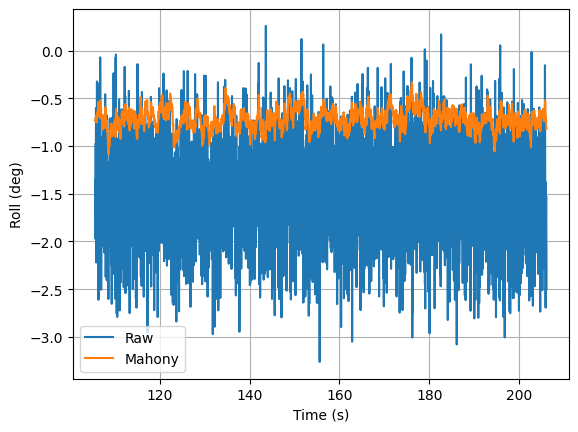
\includegraphics[width=0.85\textwidth]{figure/roll_idle_graph.png} 
    \caption{Perbandingan Respon Roll: Raw Data (Biru) vs Mahony Filter (Oranye) pada Kondisi Diam}
    \label{fig:4.roll_comparison}
\end{figure}

\begin{figure}[H]
    \centering
    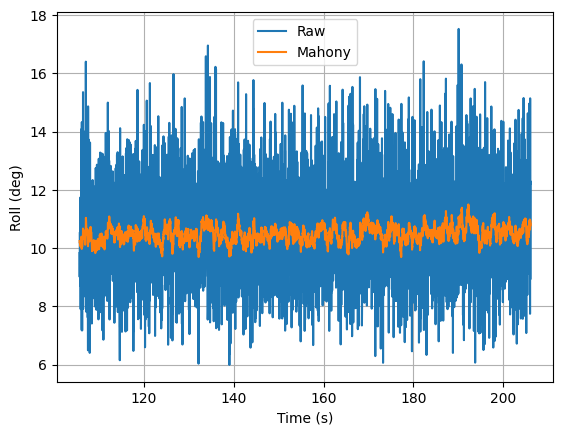
\includegraphics[width=0.85\textwidth]{figure/pitch_idle_graph.png} 
    \caption{Perbandingan Respon Pitch: Raw Data (Biru) vs Mahony Filter (Oranye) pada Kondisi Diam}
    \label{fig:4.pitch_comparison}
\end{figure}

\subsection{Pengujian Akurasi Penunjukan (\textit{Pointing Accuracy})} \label{IV.UjiPointing}
Pengujian lapangan dilakukan dengan mengarahkan teleskop ke empat objek referensi utama yang Anda gunakan, yaitu: Matahari, Bulan, Planet Jupiter, dan Bintang Betelgeuse. Koordinat target dapat diperoleh dari perangkat lunak planetarium (mis. Stellarium) menggunakan lokasi dan waktu pengujian. \par

Untuk analisis yang lebih kuat, pengujian disarankan dilakukan dalam beberapa pengulangan (mis. $n=3$ atau $n=5$ kali per objek). Dengan demikian, dapat dihitung rata-rata error dan standar deviasi error yang menggambarkan akurasi dan repeatabilitas sistem.

\begin{longtable}{|c|l|c|c|c|c|}
    \caption{Data Hasil Pengujian Penunjukan Objek Langit}
    \label{table:4.pointing_data} \\
    \hline
    \textbf{No} & \textbf{Objek} & \textbf{Target (Az/Alt)} & \textbf{Terukur (Az/Alt)} & \textbf{Error ($\Delta$)} & \textbf{Hasil Visual} \\
    \hline
    \endfirsthead
    \hline
    \textbf{No} & \textbf{Objek} & \textbf{Target (Az/Alt)} & \textbf{Terukur (Az/Alt)} & \textbf{Error ($\Delta$)} & \textbf{Hasil Visual} \\
    \hline
    \endhead
    \hline
    \endfoot
    \hline
    \endlastfoot

    1 & Matahari & $Az_t/Alt_t$ & $Az_m/Alt_m$ & $\Delta Az/\Delta Alt$ & \textbf{[Hit/Miss]} \\ \hline
    2 & Bulan & $Az_t/Alt_t$ & $Az_m/Alt_m$ & $\Delta Az/\Delta Alt$ & \textbf{[Hit/Miss]} \\ \hline
    3 & Jupiter & $Az_t/Alt_t$ & $Az_m/Alt_m$ & $\Delta Az/\Delta Alt$ & \textbf{[Hit/Miss]} \\ \hline
    4 & Betelgeuse & $Az_t/Alt_t$ & $Az_m/Alt_m$ & $\Delta Az/\Delta Alt$ & \textbf{[Hit/Miss]} \\ \hline
\end{longtable}

\subsection{Pengujian Pelacakan Objek (\textit{Tracking})} \label{IV.UjiTracking}
Pengujian \textit{tracking} bertujuan mengevaluasi kemampuan sistem mempertahankan objek tetap berada di sekitar pusat bidang pandang ketika koordinat Alt/Az target berubah terhadap waktu. Pada implementasi, pembaruan target dilakukan dengan menghitung ulang posisi objek berdasarkan waktu terkini, kemudian mengoreksi sudut motor jika selisih melebihi toleransi. \par

Skenario uji yang disarankan:
\begin{enumerate}[noitemsep]
    \item Pilih satu target (mis. Bulan/Jupiter) dan lakukan penunjukan awal hingga objek terlihat (\textit{Hit}).
    \item Jalankan \textit{tracking} selama durasi $T=\textbf{[isi menit]}$.
    \item Catat sudut target (Az/Alt), sudut terukur (encoder), serta status visual objek pada interval tetap (mis. setiap 10--30 detik).
\end{enumerate}

\begin{longtable}{|c|c|c|c|c|l|}
    \caption{Template Data Pengujian \textit{Tracking}}
    \label{table:4.tracking_data} \\
    \hline
    \textbf{No} & \textbf{Waktu (s)} & \textbf{Target (Az/Alt)} & \textbf{Terukur (Az/Alt)} & \textbf{Error} & \textbf{Catatan Visual} \\
    \hline
    \endfirsthead
    \hline
    \textbf{No} & \textbf{Waktu (s)} & \textbf{Target (Az/Alt)} & \textbf{Terukur (Az/Alt)} & \textbf{Error} & \textbf{Catatan Visual} \\
    \hline
    \endhead
    \hline
    \endfoot
    \hline
    \endlastfoot

    1 & $t_1$ & $Az_t/Alt_t$ & $Az_m/Alt_m$ & $\Delta Az/\Delta Alt$ & \textbf{[Hit/Miss]} \\ \hline
    2 & $t_2$ & $Az_t/Alt_t$ & $Az_m/Alt_m$ & $\Delta Az/\Delta Alt$ & \textbf{[Hit/Miss]} \\ \hline
\end{longtable}

\subsection{Pengujian Mode Manual (\textit{Slew})} \label{IV.UjiManual}
Pengujian mode manual dilakukan untuk memverifikasi bahwa teleskop dapat digerakkan secara langsung oleh pengguna (mis. tombol arah pada aplikasi) untuk koreksi halus saat \textit{setup} dan \textit{alignment}. Uji mencakup arah gerak, konsistensi respons, dan kestabilan setelah motor berhenti. \par

\begin{table}[H]
    \centering
    \caption{Template Hasil Uji Mode Manual (Slew)}
    \label{table:4.manual_test}
    \begin{tabular}{|l|c|c|p{0.44\textwidth}|}
    \hline
    \textbf{Aksi} & \textbf{Arah Benar} & \textbf{Respons (ms)} & \textbf{Catatan} \\ \hline
    Kiri (Az--) & \textbf{[Ya/Tidak]} & \textbf{[isi]} & \textbf{[isi]} \\ \hline
    Kanan (Az++) & \textbf{[Ya/Tidak]} & \textbf{[isi]} & \textbf{[isi]} \\ \hline
    Atas (Alt++) & \textbf{[Ya/Tidak]} & \textbf{[isi]} & \textbf{[isi]} \\ \hline
    Bawah (Alt--) & \textbf{[Ya/Tidak]} & \textbf{[isi]} & \textbf{[isi]} \\ \hline
    \end{tabular}
\end{table}

\subsection{Pengujian Komunikasi Real-Time (WebSocket)} \label{IV.UjiWebSocket}
Pengujian ini memastikan pertukaran data antara aplikasi Android dan ESP32 berjalan real-time melalui WebSocket, mencakup koneksi awal, pengiriman perintah (mis. \textit{goto-star}, \textit{goto-planet}, dan \textit{slew} manual), serta penerimaan status posisi. \par

Parameter yang dapat diukur meliputi \textit{round-trip time} (RTT), tingkat \textit{packet loss} (jika ada), serta perilaku \textit{reconnect}. Jika tidak tersedia pengukuran kuantitatif, uraikan bukti fungsional (tangkapan layar/log serial). \par

\begin{table}[H]
    \centering
    \caption{Template Hasil Uji WebSocket}
    \label{table:4.websocket_test}
    \begin{tabular}{|p{0.36\textwidth}|c|p{0.5\textwidth}|}
    \hline
    \textbf{Skenario} & \textbf{Hasil} & \textbf{Catatan/Bukti} \\ \hline
    Koneksi awal aplikasi--ESP32 & \textbf{[OK/Gagal]} & \textbf{[isi]} \\ \hline
    Kirim perintah GoTo (bintang/planet/bulan/matahari) & \textbf{[OK/Gagal]} & \textbf{[isi]} \\ \hline
    Terima status posisi (Az/Alt) periodik & \textbf{[OK/Gagal]} & \textbf{[isi]} \\ \hline
    Putus--sambung (reconnect) & \textbf{[OK/Gagal]} & \textbf{[isi]} \\ \hline
    \end{tabular}
\end{table}

\subsection{Pengujian Tampilan Status pada Antarmuka} \label{IV.UjiUI}
Pengujian antarmuka bertujuan memastikan aplikasi menampilkan informasi yang diperlukan pengguna, seperti mode operasi, status koneksi, posisi terukur (Az/Alt dari encoder), serta target yang sedang diproses. Bukti dapat berupa tangkapan layar dan deskripsi elemen UI. \par

\subsection{Pengujian Logging / Penyimpanan Data} \label{IV.UjiLogging}
Jika sistem menyediakan \textit{logging} (mis. via serial monitor, penyimpanan lokal aplikasi, atau file), pengujian dilakukan untuk memverifikasi format data, konsistensi penulisan, dan kemudahan ekstraksi untuk analisis. Jika fitur ini belum diimplementasikan, subbab ini dapat diisi sebagai \textit{evaluasi} dan rencana pengembangan. \par

\subsection{Pengujian Indikator Error, Batas, dan Koneksi} \label{IV.UjiErrorIndicator}
Pengujian ini mengevaluasi bagaimana sistem memberi umpan balik ketika terjadi kondisi abnormal, seperti koneksi terputus, perintah target tidak valid, atau sudut target melewati batas mekanik yang aman. Uraikan indikator yang tersedia (mis. pesan di aplikasi/log serial) dan hasil uji skenario tersebut. \par

\subsection{Pengujian Frekuensi Pembaruan Sensor (Target 100~Hz)} \label{IV.UjiFreq}
Pengujian ini bertujuan mengonfirmasi bahwa \textit{task} sensor berjalan mendekati target 100~Hz. Cara uji yang disarankan adalah mencatat interval waktu $dt$ pada log (serial) selama durasi tertentu, lalu menghitung $f_s = 1/\overline{dt}$. \par

\subsection{Pengujian Keandalan saat Koneksi Terputus} \label{IV.UjiReliabilityDisconnect}
Pengujian ini memverifikasi kebutuhan non-fungsional terkait keandalan: ketika koneksi terputus, sistem harus tetap aman dan dapat dikendalikan melalui mode manual (fallback). Skenario uji: putuskan WiFi saat motor bergerak/diam, amati reaksi sistem, lalu uji apakah kontrol manual masih dapat dijalankan. \par

\section{Analisis dan Pembahasan} \label{IV.Analisis}

Bagian ini menganalisis temuan dari hasil pengujian dengan menautkan data sensor, logika kontrol, serta faktor mekanik yang mempengaruhi hasil observasi. \par

\subsection{Objektif Evaluasi dan Kriteria Keberhasilan} \label{IV.Objektif}
Objektif evaluasi pada Bab IV dirumuskan agar hasil pengujian dapat dinilai secara terukur:
\begin{enumerate}[noitemsep]
    \item \textbf{Objektif-1 (Stabilitas sensor)}: keluaran \textit{pitch/roll} dari IMU menjadi stabil (nilai $\sigma$ menurun) setelah Mahony Filter diterapkan \cite{Mahony2007,Alfian2021}.
    \item \textbf{Objektif-2 (Referensi arah \textit{azimuth})}: sistem dapat memiliki referensi \textit{azimuth} absolut yang konsisten melalui inisialisasi kompas (tilt-compensated heading) sebelum menggunakan encoder sebagai pembacaan operasional.
    \item \textbf{Objektif-3 (Akurasi penunjukan)}: teleskop mampu diarahkan ke objek referensi (Matahari, Bulan, Jupiter, Betelgeuse) dengan error yang dapat dijelaskan dan direduksi melalui kalibrasi dan koreksi mekanik.
\end{enumerate}

\subsection{Analisis Stabilitas Sensor Berbasis Standar Deviasi} \label{IV.AnalisisSigma}
Nilai standar deviasi pada Tabel \ref{table:4.noise_stats} digunakan untuk memisahkan dua fenomena: (1) \textit{noise} acak berfrekuensi tinggi (muncul sebagai jitter), dan (2) \textit{drift}/bias lambat yang menyebabkan pembacaan bergeser. Mahony Filter menekan \textit{noise} pada \textit{pitch/roll} dengan memanfaatkan vektor gravitasi sebagai koreksi terhadap giroskop \cite{Mahony2007}. \par

Dalam implementasi, pembaruan Mahony hanya dilakukan ketika norm akselerasi berada pada rentang tertentu (untuk menolak data yang terkontaminasi percepatan non-gravitasi). Mekanisme ini menjaga filter tidak ``terkunci'' pada data akselerometer yang tidak valid saat terjadi gerakan cepat. \par

Untuk encoder AS5600, fluktuasi kecil yang terlihat pada data \textit{altitude/azimuth} umumnya berasal dari kuantisasi resolusi 12-bit. Dengan resolusi sudut per hitungan sebesar $\approx 0.088^{\circ}$, standar deviasi pada encoder seringkali kecil namun tidak nol, terutama jika terdapat getaran mekanik yang membuat sensor melewati batas hitungan bolak-balik. \par

\subsection{Analisis Akurasi Penunjukan: Error Sudut dan Repeatabilitas} \label{IV.AnalisisPointing}
Untuk setiap percobaan penunjukan, error sudut pada dua sumbu dihitung sebagai:
\begin{equation}
\Delta Az = wrap\left(Az_m - Az_t\right), \quad \Delta Alt = Alt_m - Alt_t
\end{equation}
dengan \textit{wrap} digunakan agar perbedaan \textit{azimuth} berada pada rentang $[-180^{\circ}, 180^{\circ}]$. \par

Jika diperlukan satu metrik gabungan (\textit{pointing error}), dapat digunakan pendekatan proyeksi lokal:
\begin{equation}
\epsilon \approx \sqrt{\left(\Delta Az\,\cos(Alt_t)\right)^2 + \left(\Delta Alt\right)^2}
\end{equation}
Metrik $\epsilon$ mempermudah perbandingan performa antar objek. Untuk pengulangan $n$ kali per objek, hitung juga $\bar{\epsilon}$ dan $\sigma_{\epsilon}$ sebagai indikator akurasi rata-rata dan repeatabilitas. \par

\subsection{Analisis Keterlihatan Objek dan Hubungan dengan FOV} \label{IV.AnalisisFOV}
Hasil \textit{Hit/Miss} tidak hanya ditentukan oleh besarnya error sudut, tetapi juga oleh ukuran semu objek dan \textit{Field of View} (FOV) sistem optik. Bulan dan Matahari memiliki diameter sudut semu sekitar $\approx 0.5^{\circ}$, sehingga toleransi error penunjukan relatif lebih besar dibanding objek titik (bintang dan planet) yang terlihat sebagai titik terang. \par

Jika diketahui \textit{apparent field of view} (AFOV) okuler dan perbesaran $M$, maka FOV dapat diperkirakan:
\begin{equation}
FOV \approx \frac{AFOV}{M}
\end{equation}
Dengan FOV yang kecil (mis. $< 1^{\circ}$), error penunjukan beberapa derajat hampir pasti menghasilkan \textit{miss}. Oleh karena itu, pengujian pada objek titik seperti Betelgeuse dan Jupiter adalah uji yang lebih ketat untuk stabilitas mekanik dan repeatabilitas arah. \par

\subsection{Analisis Offset dan Kalibrasi Satu Bintang (\textit{One-Star Alignment})} \label{IV.AnalisisAlignment}
Hasil observasi Anda menunjukkan adanya \textit{miss} pada beberapa target. Secara praktis, pendekatan yang umum pada sistem biaya rendah adalah melakukan kalibrasi offset menggunakan satu objek referensi (mis. Betelgeuse). Setelah teleskop berhasil diarahkan secara manual hingga objek berada di pusat FOV, offset dihitung:
\begin{equation}
\delta_{Az} = Az_t - Az_m, \quad \delta_{Alt} = Alt_t - Alt_m
\end{equation}
Kemudian koreksi diterapkan untuk perintah berikutnya:
\begin{equation}
Az_{cmd} = Az_t + \delta_{Az}, \quad Alt_{cmd} = Alt_t + \delta_{Alt}
\end{equation}
Metode ini efektif untuk mengurangi error sistematis yang konstan pada rentang sudut tertentu, namun tidak sepenuhnya mengatasi error yang bergantung pada posisi (mis. flex yang berubah saat altitude tinggi). \par

\subsection{Analisis Faktor Mekanik: \textit{Rigidity}, \textit{Backlash}, dan Getaran} \label{IV.AnalisisMekanik}
Walaupun perhitungan sudut target telah tepat, performa optik akhirnya sangat dipengaruhi oleh mekanik. Struktur cetak 3D cenderung memiliki flex mikro. Saat motor berhenti, energi inersia OTA dapat memicu osilasi kecil yang menyebabkan sumbu optik bergeser, sehingga objek titik (Jupiter dan Betelgeuse) mudah keluar dari FOV. Fenomena serupa dilaporkan pada instrumen \textit{low-cost} untuk pengamatan hilal yang objeknya tidak selalu berada di tengah bidang pandang \cite{Hadi2022}. \par

Selain flex, \textit{backlash} pada transmisi (gear/belt) dan toleransi pemasangan juga memunculkan error arah yang bergantung pada arah gerak (histeresis). Untuk menguji ini, lakukan skenario yang sama dengan dua arah pendekatan: mendekati target dari arah kiri dan kanan, lalu bandingkan selisih sudut akhir. \par

\subsection{Analisis \textit{Error Budget} Sistem} \label{IV.ErrorBudget}
Untuk memahami prioritas perbaikan, error total dapat dipandang sebagai kombinasi beberapa komponen: 
\begin{enumerate}[noitemsep]
    \item \textbf{Error sensor (acak)}: direpresentasikan oleh $\sigma$ pada IMU/kompas/encoder.
    \item \textbf{Error sensor (sistematis)}: offset kalibrasi \textit{pitchCorrection}, \textit{rollCorrection}, \textit{altitudeOffset}, serta referensi \textit{deltaAzimuth}.
    \item \textbf{Error mekanik}: flex, backlash, misalignment antara sumbu sensor dan sumbu optik.
    \item \textbf{Error observasi}: getaran angin, kualitas tripod/permukaan, dan kesalahan penilaian \textit{Hit/Miss} oleh operator.
\end{enumerate}

Sebagai contoh, resolusi encoder AS5600 (12-bit) memberi batas kuantisasi $\approx 0.088^{\circ}$ per langkah. Namun pada praktiknya, error mekanik seringkali lebih dominan daripada kuantisasi. Tabel berikut disediakan sebagai template untuk menyusun ringkasan error yang Anda temukan.

\begin{table}[H]
    \centering
    \caption{Template Ringkasan Komponen Error (Error Budget)}
    \label{table:4.error_budget}
    \begin{tabular}{|p{0.42\textwidth}|p{0.18\textwidth}|p{0.32\textwidth}|}
    \hline
    \textbf{Sumber Error} & \textbf{Besaran} & \textbf{Cara Estimasi} \\ \hline
    Kuantisasi encoder AS5600 & $\approx 0.088^{\circ}$ & $360/4096$ \\ \hline
    \textit{Noise} pitch/roll (IMU) & $\sigma_{filt,pitch},\sigma_{filt,roll}$ & std dev saat \textit{static test} \\ \hline
    \textit{Noise} heading (kompas) & $\sigma_{head}$ & std dev \textit{heading} terkompensasi tilt \\ \hline
    Backlash/flex mekanik & $\Delta_{mech}$ & beda hasil saat pendekatan dua arah \\ \hline
    Misalignment sensor-optik & $\Delta_{align}$ & offset konsisten setelah \textit{one-star alignment} \\ \hline
    \end{tabular}
\end{table}

\subsection{Evaluasi Sistem Penggerak dan Implikasi \textit{Open-Loop}} \label{IV.AnalisisMotor}
Motor stepper NEMA 17 dengan driver A4988 memberikan gerakan halus, terutama ketika \textit{microstepping} diaktifkan. Namun, karena kontrol stepper bersifat \textit{open-loop}, sistem tidak dapat mendeteksi \textit{missed step} secara langsung. Pada desain Anda, penggunaan encoder AS5600 membantu menyediakan pembacaan sudut aktual pada masing-masing sumbu, sehingga koreksi dapat dilakukan berdasarkan error sudut, bukan semata jumlah langkah. Pendekatan ini meningkatkan robusta sistem dibanding stepper murni tanpa sensor posisi. \par

\subsection{Ringkasan Analisis} \label{IV.Ringkasan}
Secara keseluruhan, Mahony Filter berhasil meningkatkan kestabilan keluaran IMU (ditunjukkan oleh penurunan $\sigma$), sementara encoder memberikan pembacaan sudut yang lebih stabil untuk operasi \textit{azimuth/altitude}. Kegagalan penunjukan yang terjadi lebih dominan berasal dari faktor mekanik (rigidity dan getaran) serta offset sistematis yang dapat diminimalkan melalui prosedur kalibrasi berbasis objek referensi. Untuk meningkatkan akurasi ke level observatorium, dibutuhkan peningkatan material/rigiditas serta skema kalibrasi kompas dan mekanik yang lebih ketat \cite{Malasan2025}. \par
